\section{Data Understanding}

The dataset contains 471910 entries, each of them represent a purchase related to a supermarket made by a customer over a period of one year.

\subsection{Data Semantics}

This dataset contains 8 attributes that correspond to:

\begin{itemize}
\item \textbf{BasketID} (\emph{24627}): a 6 digit integer number uniquely assigned to each purchase; if it starts with a \emph{C}, it indicates a cancellation (\emph{3754});
\item \textbf{BasketDate}: the day (\emph{from 2010/12/01 to 2011/12/09}) and time (\emph{from 6am to 21pm}) when each purchase was placed;
\item \textbf{Sale} (\emph{∼4avg}): the unit product price, all in the same currency, probably in sterling;
\item \textbf{CustomerID} (\emph{4372 + 65073na}): a 5 digit integer number uniquely assigned to each customer;
\item \textbf{CustomerCountry} (\emph{37}): the name of the country where each customer resides;
\item \textbf{ProdID} (\emph{3953}): a 5 digit + 1 letter identifier uniquely assigned to each distinct product; identical codes with different letters identify the same products with different characteristics (\emph{e.g.}, 84997D: '\emph{pink piece polkadot cutlery set} vs. 84997C: '\emph{blue piece polkadot cutlery set});
\item \textbf{ProdDescr} (\emph{4097 + 753na}): the description of the product purchased;
\item \textbf{Qta} (\emph{∼11avg}): the purchased quantities of each product per order.
\end{itemize}

\subsection{Assessing Data Quality}
In order to assess the quality of data, we proceed by removing the \emph{5232} duplicate entries, so we will work with the remaining \emph{466678} rows.

Then, we proceed by removing the entries corresponding to the \emph{65073} null \emph{CustomerID} values, since there is no way to integrate them to trace the original customer.

Afterwards, we checked the \emph{ProdID} that does not respect the defined format and we found some that contains only letters, \emph{e.g.}, '\emph{POST}', '\emph{D}', '\emph{C2}', '\emph{M}', '\emph{BANK CHARGES}', etc. with the following respective \emph{ProdDescr}: '\emph{POSTAGE}', '\emph{Discount}', '\emph{CARRIAGE}', '\emph{Manual}', '\emph{Bank Charges}'.

\begin{wrapfigure}{r}{.5\textwidth}
\centering
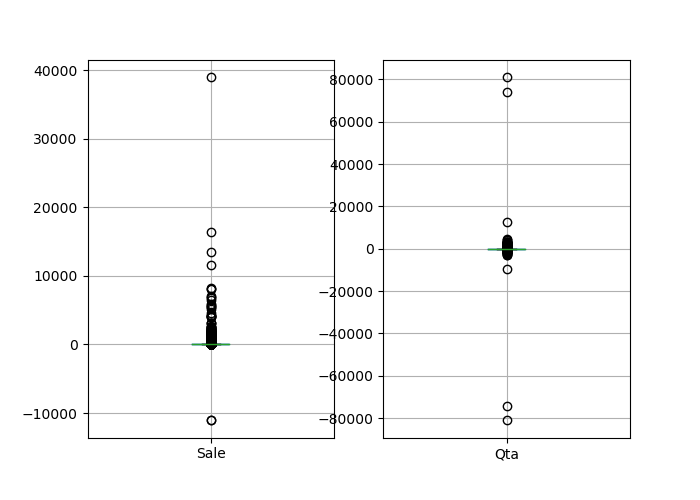
\includegraphics[width=0.49\textwidth]{img/boxplot_before.png}
\caption{Box Plot for outliers detection}
\end{wrapfigure}

For what regards the outliers, we used a box plot to visualize the two continuous attributes that we have, that are \textbf{Sale} and \textbf{Qta}.\\
From these plots, we found that, for both attributes, the box is very flat, meaning that the vast majority of the values fall in a small range. Nevertheless, there are several outliers, someone with a value really far away from the median; these values could represent an issue for the analysis we will perform. Plus, here we can notice the negative values we already found during the semantic analysis.

\subsection{Variables Transformations}
We chosen to categorize the attribute \textbf{BasketDate}, by first splitting the date information and the time information, and then

\begin{itemize}
\item for the time, we decided to divide the day hours into 5 categories:
	\begin{itemize}
	\item \emph{Early morning}, from 6 to 9;
	\item \emph{Morning}, from 9 to 12;
	\item \emph{Lunch time}, from 12 to 15;
	\item \emph{Evening}, from 15 to 18;
	\item \emph{Late evening}, from 18 to 21.
	\end{itemize}
\item for the date, we chosen to keep the week of the transaction.
\end{itemize}

The rationale behind these choices is that we are more interested in the period in which a transaction occurs, rather that its precise date and time, to be able to cluster customers with a similar shopping behavior; furthermore, since the dataset is not from a grocery store, the customers with several shopping sessions per day or per week are really rare, and so we decided to use a broader partitioning.\\
After these categorization, we ended up introducing \textbf{DayTime} and \textbf{Week}.

We also decided to create the attribute \textbf{TotalPrice}, which is simply the product of \textbf{Sale} and \textbf{Qta}, and represents the total amount spent by a customer for each record. We made this choice mainly to have a clearer look to the dataset, emphasizing an important information that was not explicit in the original table, and also to simplify the extraction of some features and statistics.

\subsection{Variables Distribution}
In this section, we will study the distribution of various attributes, by plotting some interesting properties about them.

\begin{figure}[!h]
\begin{subfigure}{.5\textwidth}
\centering
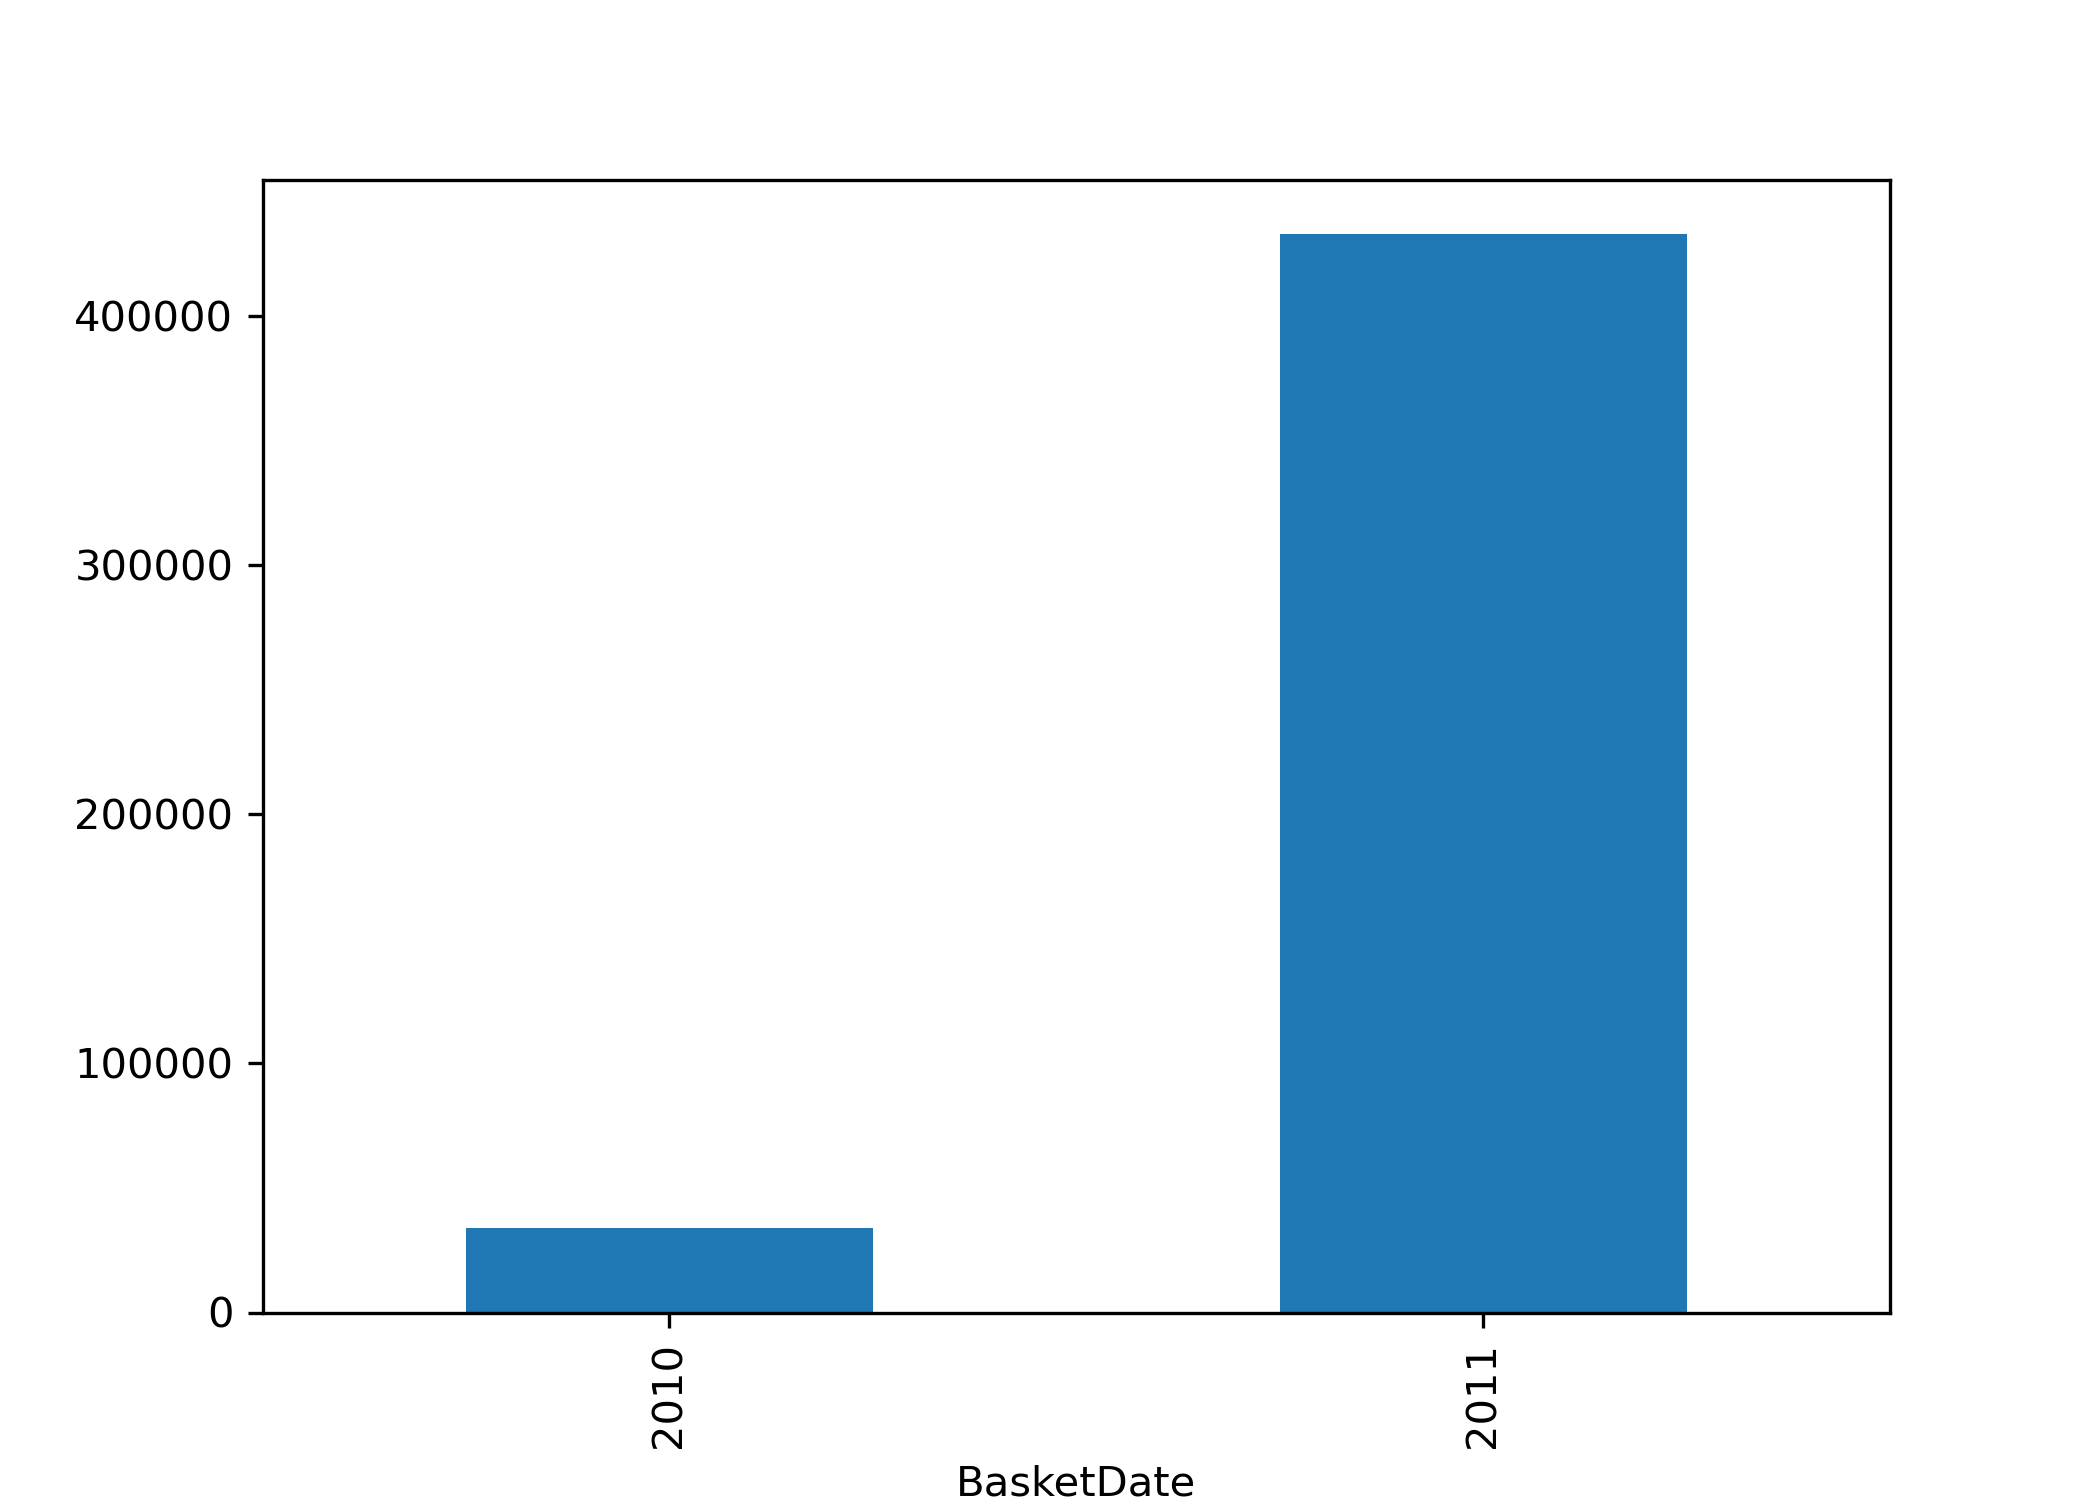
\includegraphics[width=.7\textwidth]{img/year_count.png}
\caption{Year}
\label{fig:year_count}
\end{subfigure}
\begin{subfigure}{.5\textwidth}
\centering
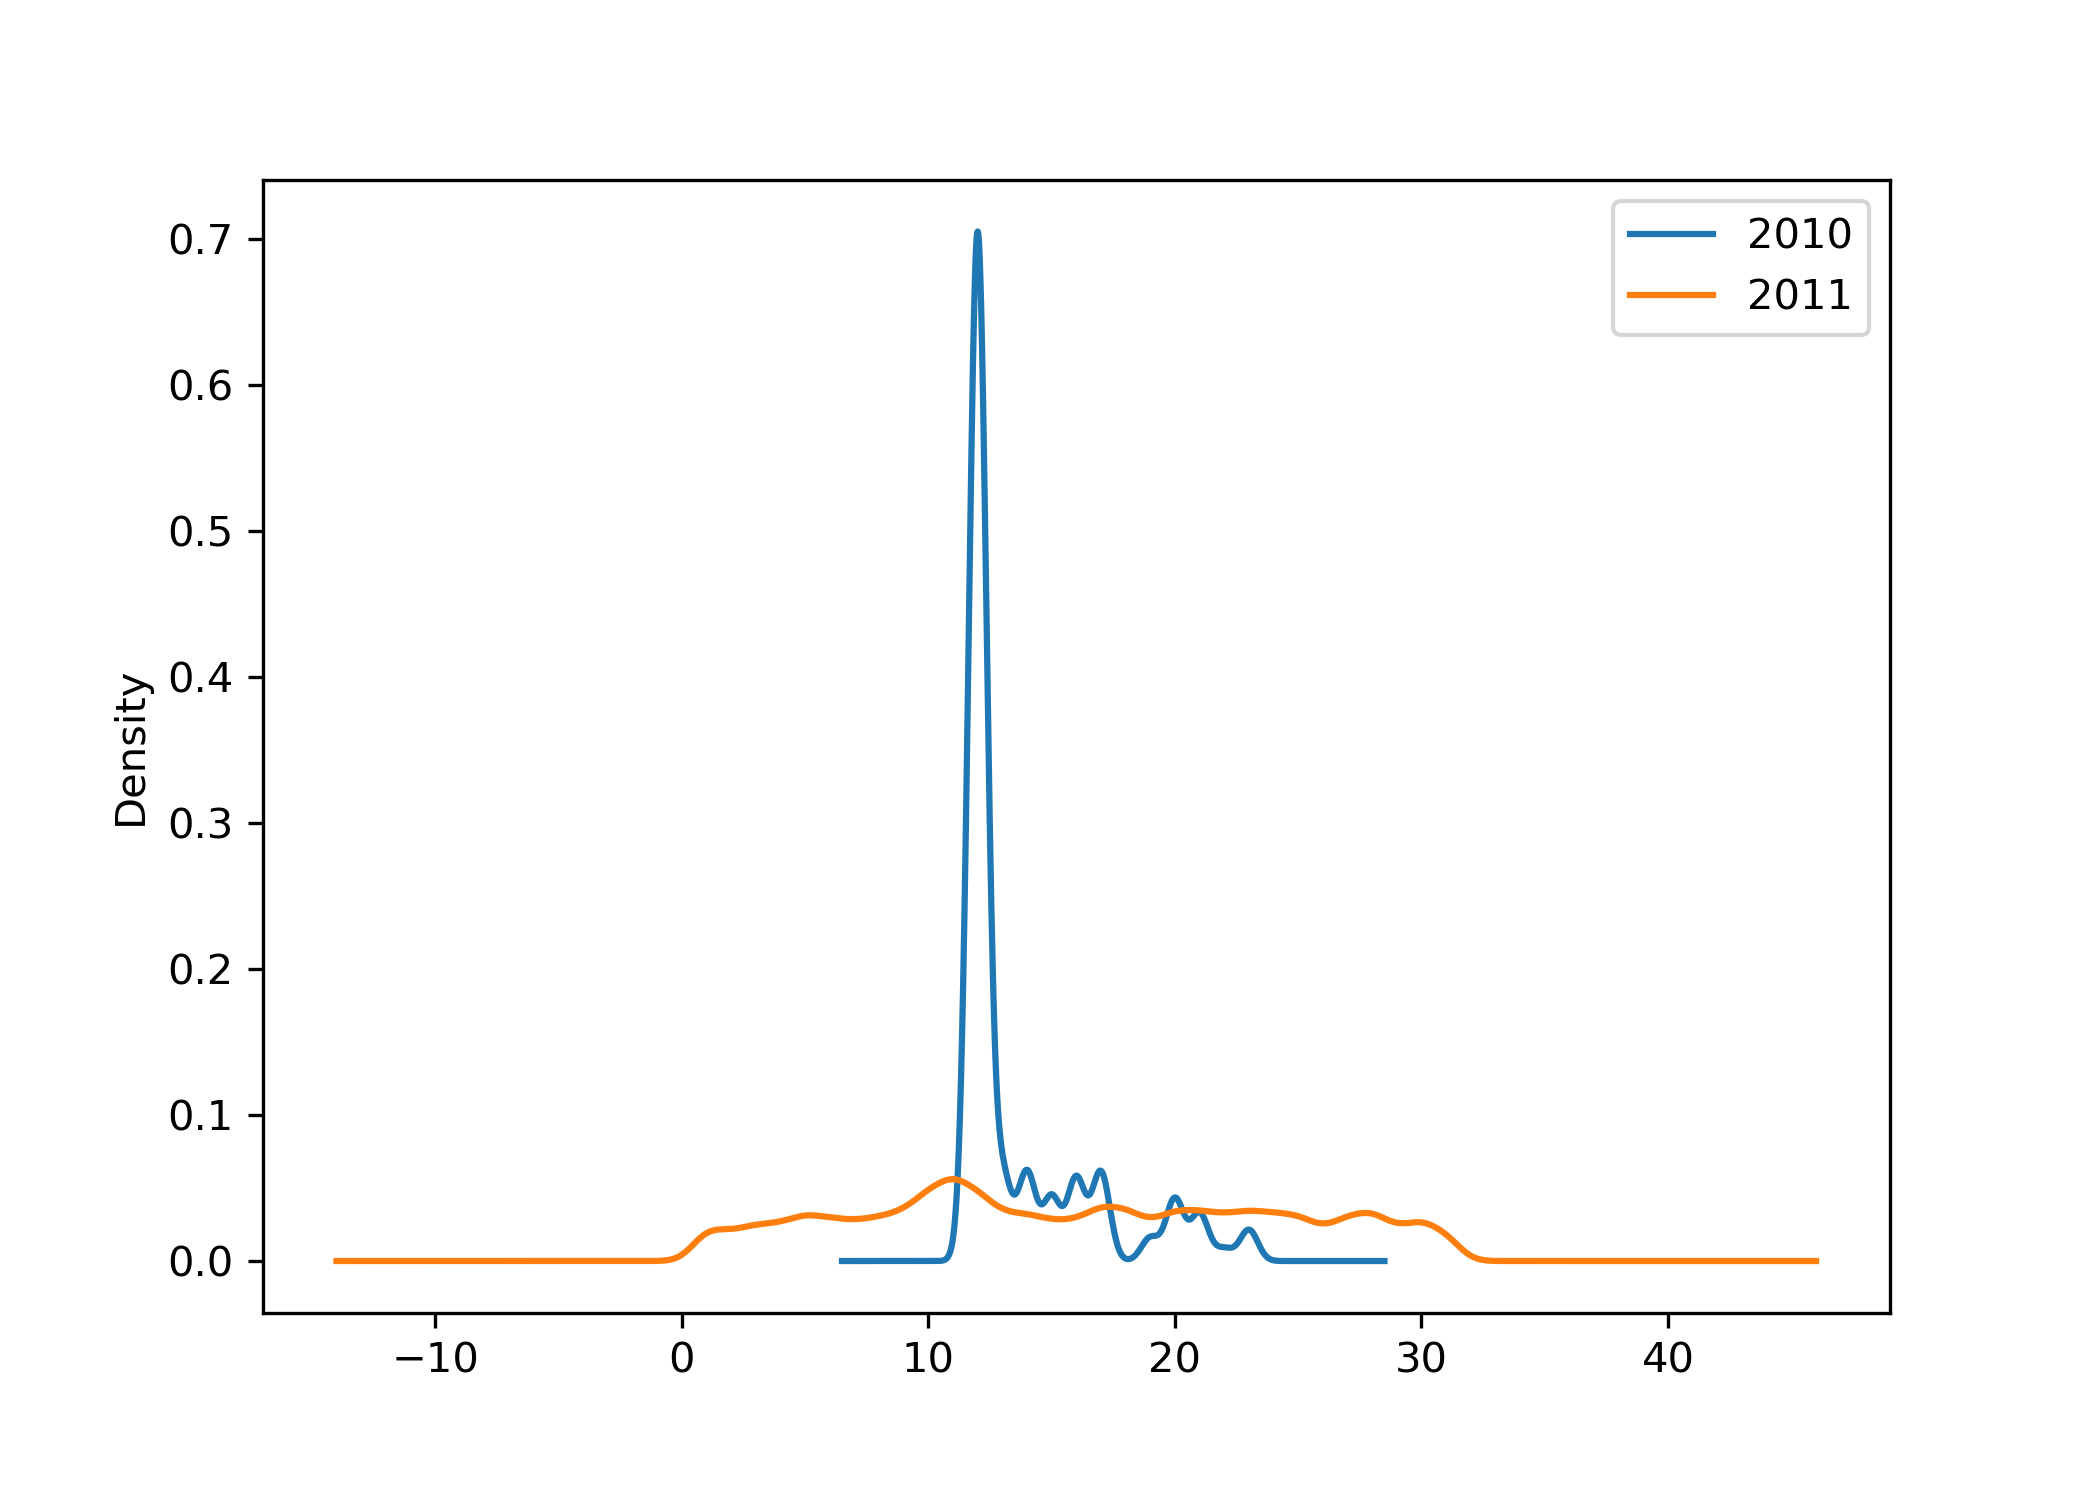
\includegraphics[width=.7\textwidth]{img/kde_year.png}
\caption{PDF by Year}
\label{fig:kde_year}
\end{subfigure}
\begin{subfigure}{.5\textwidth}
\centering
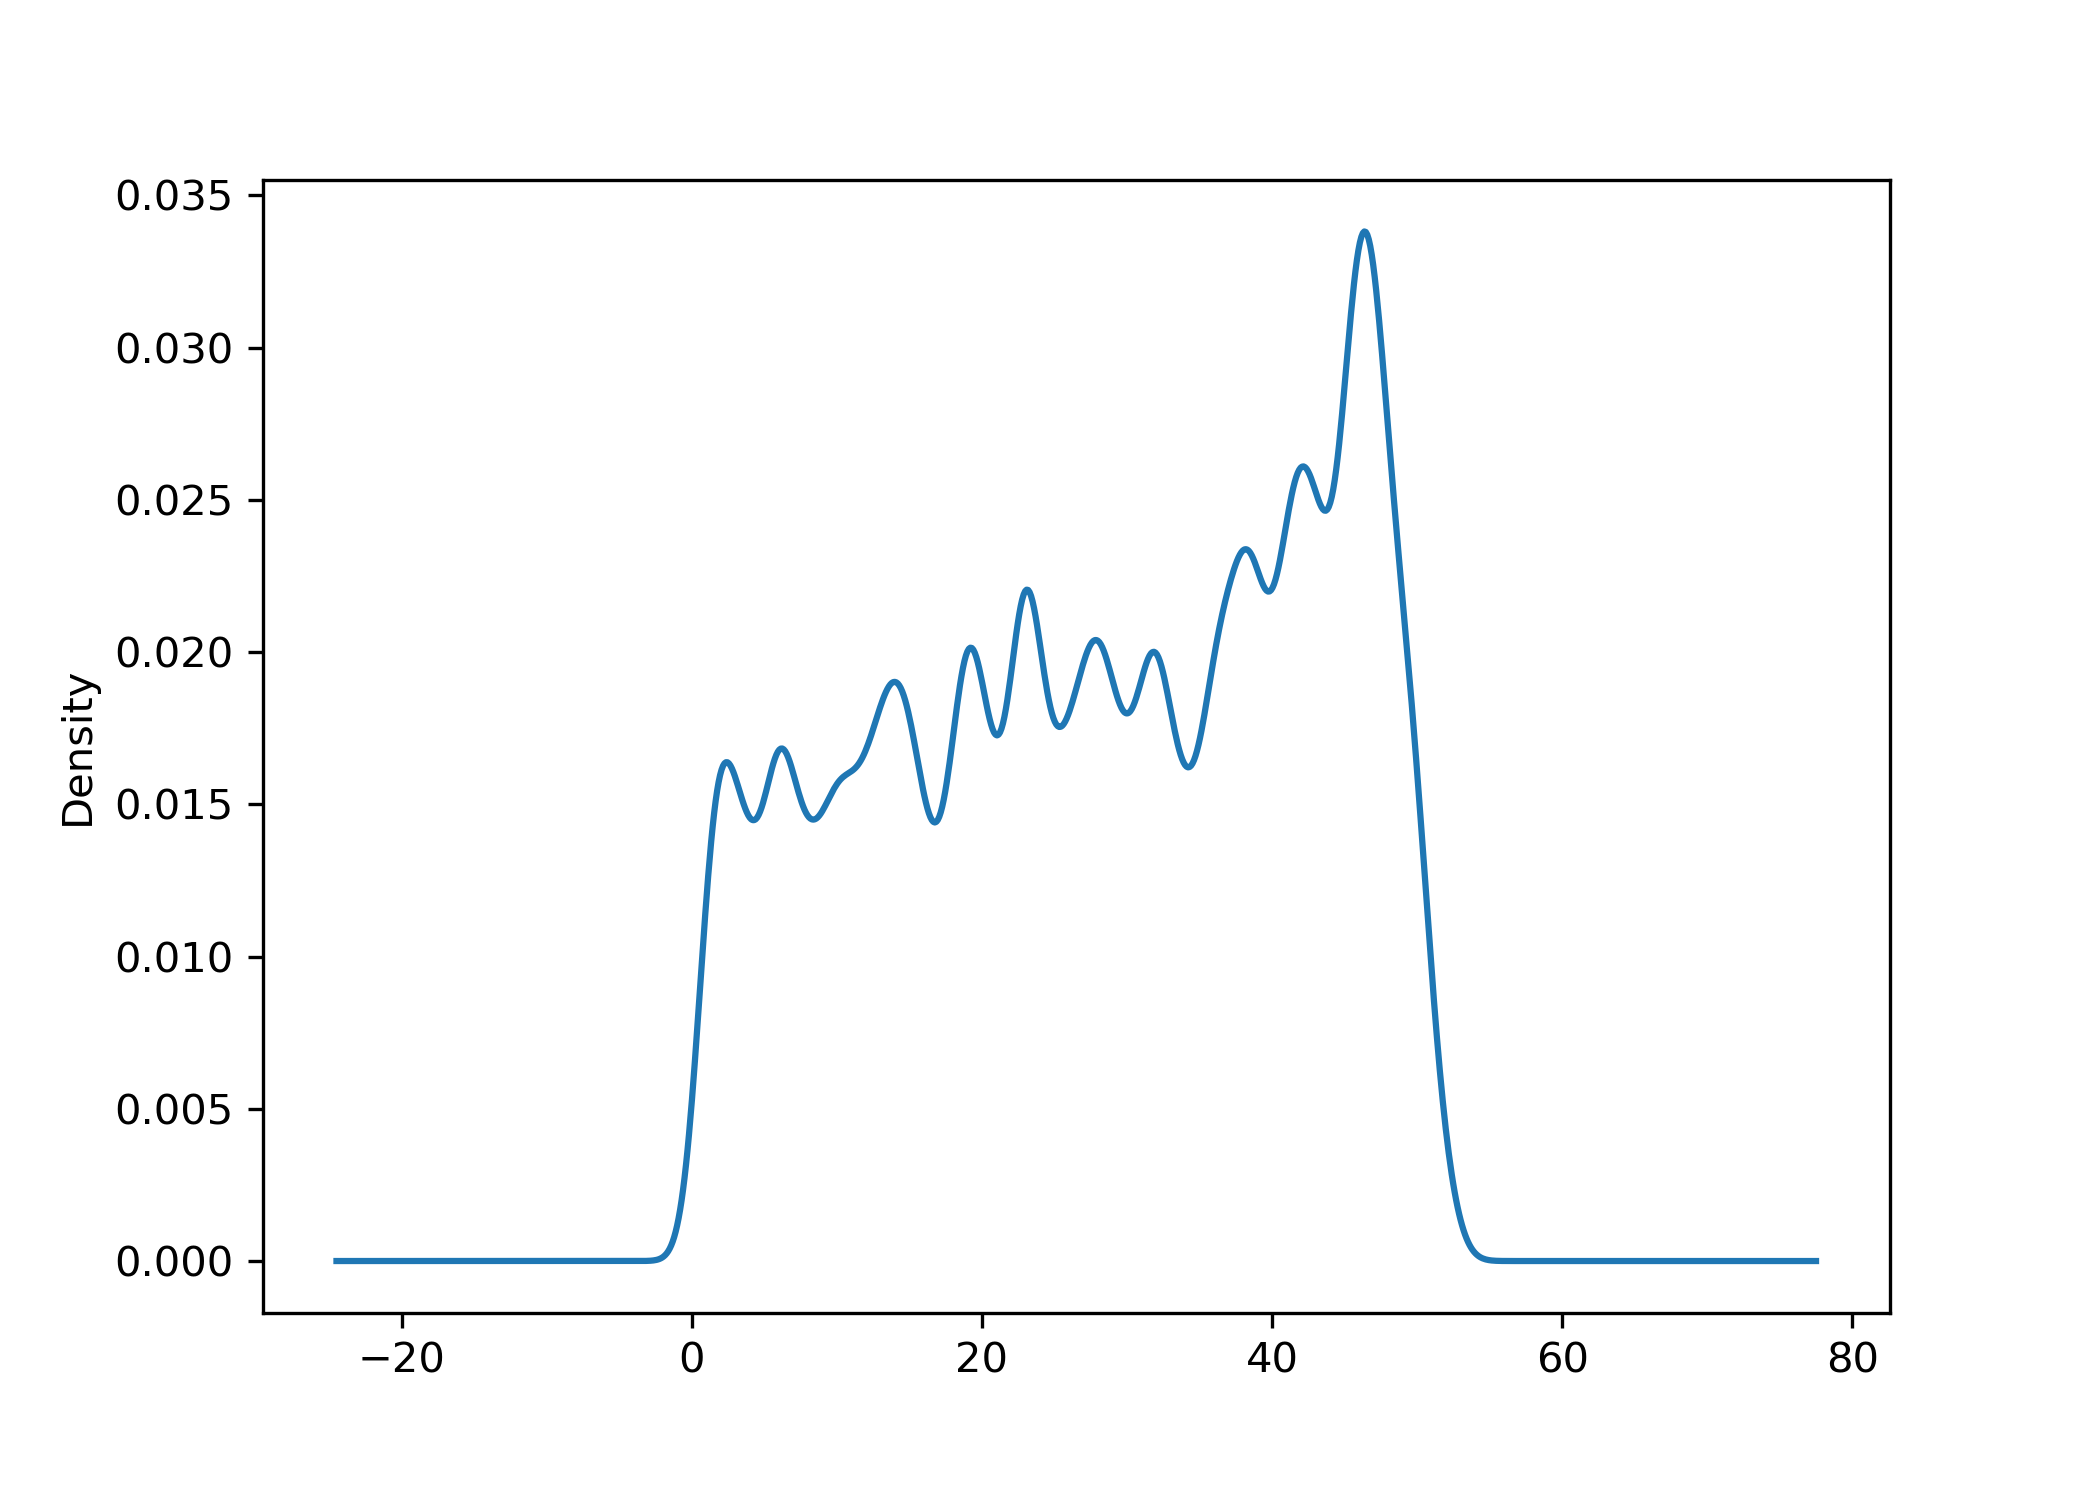
\includegraphics[width=.7\textwidth]{img/week_kde.png}
\caption{PDF by Week}
\label{fig:week_kde}
\end{subfigure}
\begin{subfigure}{.5\textwidth}
\centering
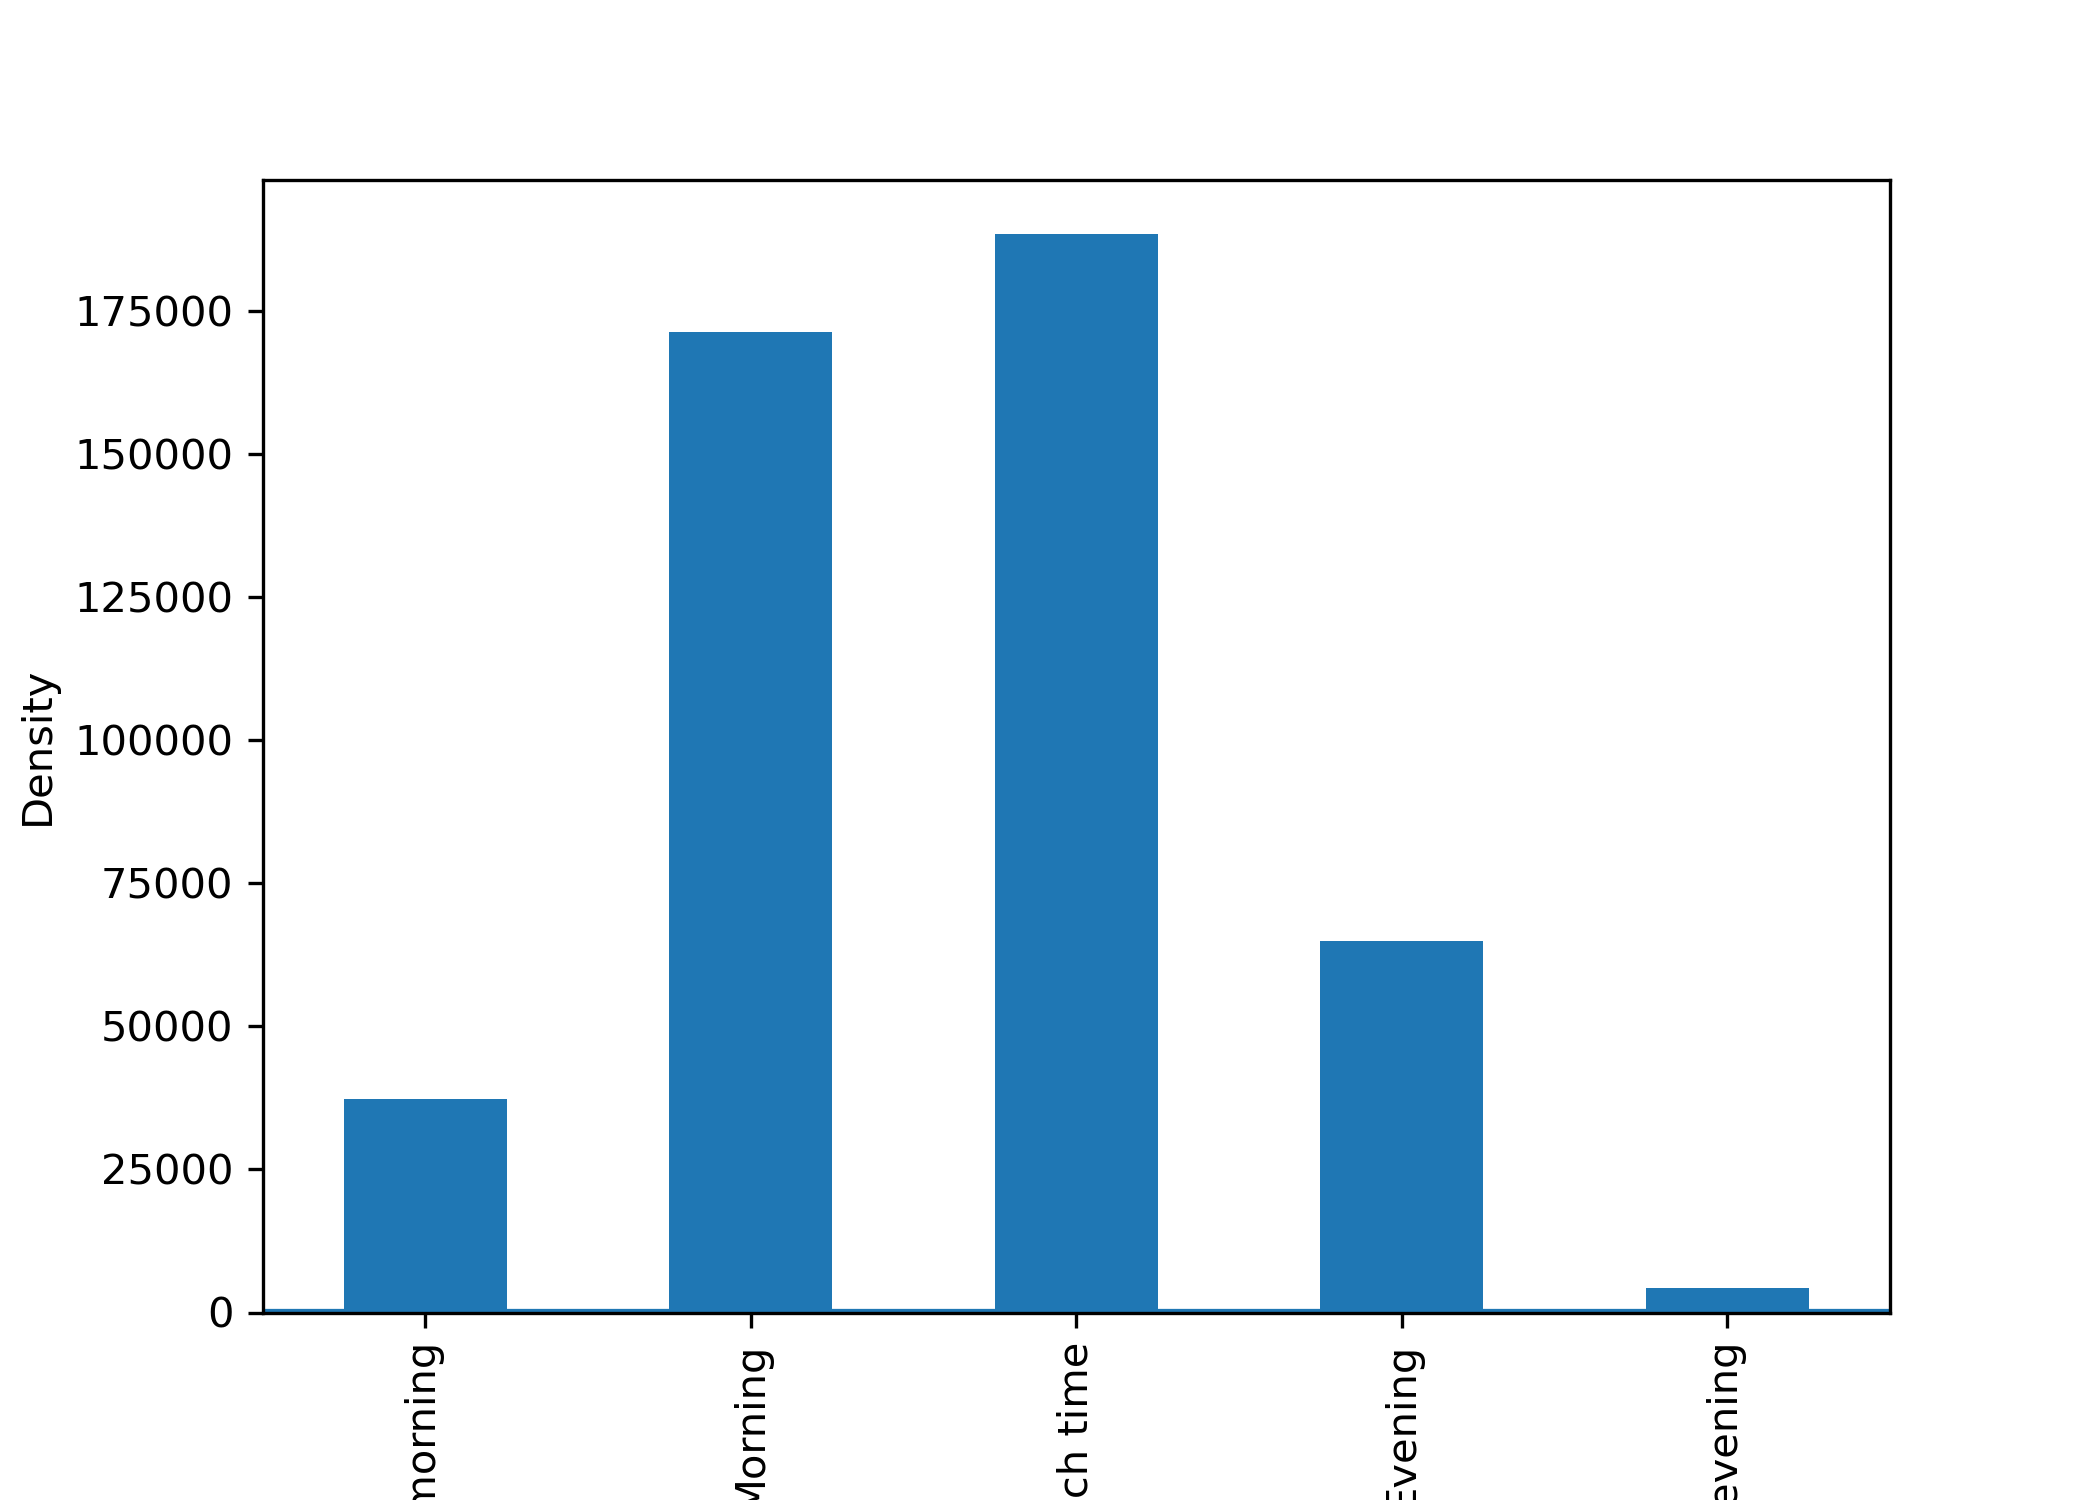
\includegraphics[width=.7\textwidth]{img/daytime_bar.png}
\caption{Day Time}
\label{fig:daytime_bar}
\end{subfigure}
\caption{BasketDate Distributions}
\end{figure}

First, we analyse the \textbf{BasketDate}.\\
From the Figure \ref{fig:year_count}, we can see that the attribute is highly unbalanced; in fact, we have that almost all the records are related to transaction of the 2011, while the objects from 2010 are very few.
Indeed, the rows of 2011 represent about the 93\% of the whole dataset.\\
Furthermore, from the Figure \ref{fig:kde_year}, that represents an estimation of the probability density function of \textbf{BasketDate} divided by year, we can appreciate the two different distributions.\\
In fact, for the 2010, we have a very uneven plot, which indicates that the records are not uniformly distributed with respect to the days in a month. This because, for the majority of the months in 2010, there were registered only transactions from a single day, the 12th; this is the value for which the plot shows the peak.\\
On the other hand, the distribution for the 2011 is much more homogeneous, meaning that the transactions were registered for most days in the months of that year.\\
Another interesting distributions are plotted in Figure \ref{fig:week_kde} and \ref{fig:daytime_bar}.\\
In the first one, we can see that the last weeks of the year are the one with more purchases; that is consistent with our expectations, since those are the weeks closest to Christmas time, that typically represents a great period of shopping.\\	
In the second one, the focus is instead on the hours in a day; we found that, unsurprisingly, the most popular hourly range goes from 9 to 18.

\begin{figure}[!h]
\begin{subfigure}{.5\textwidth}
\centering
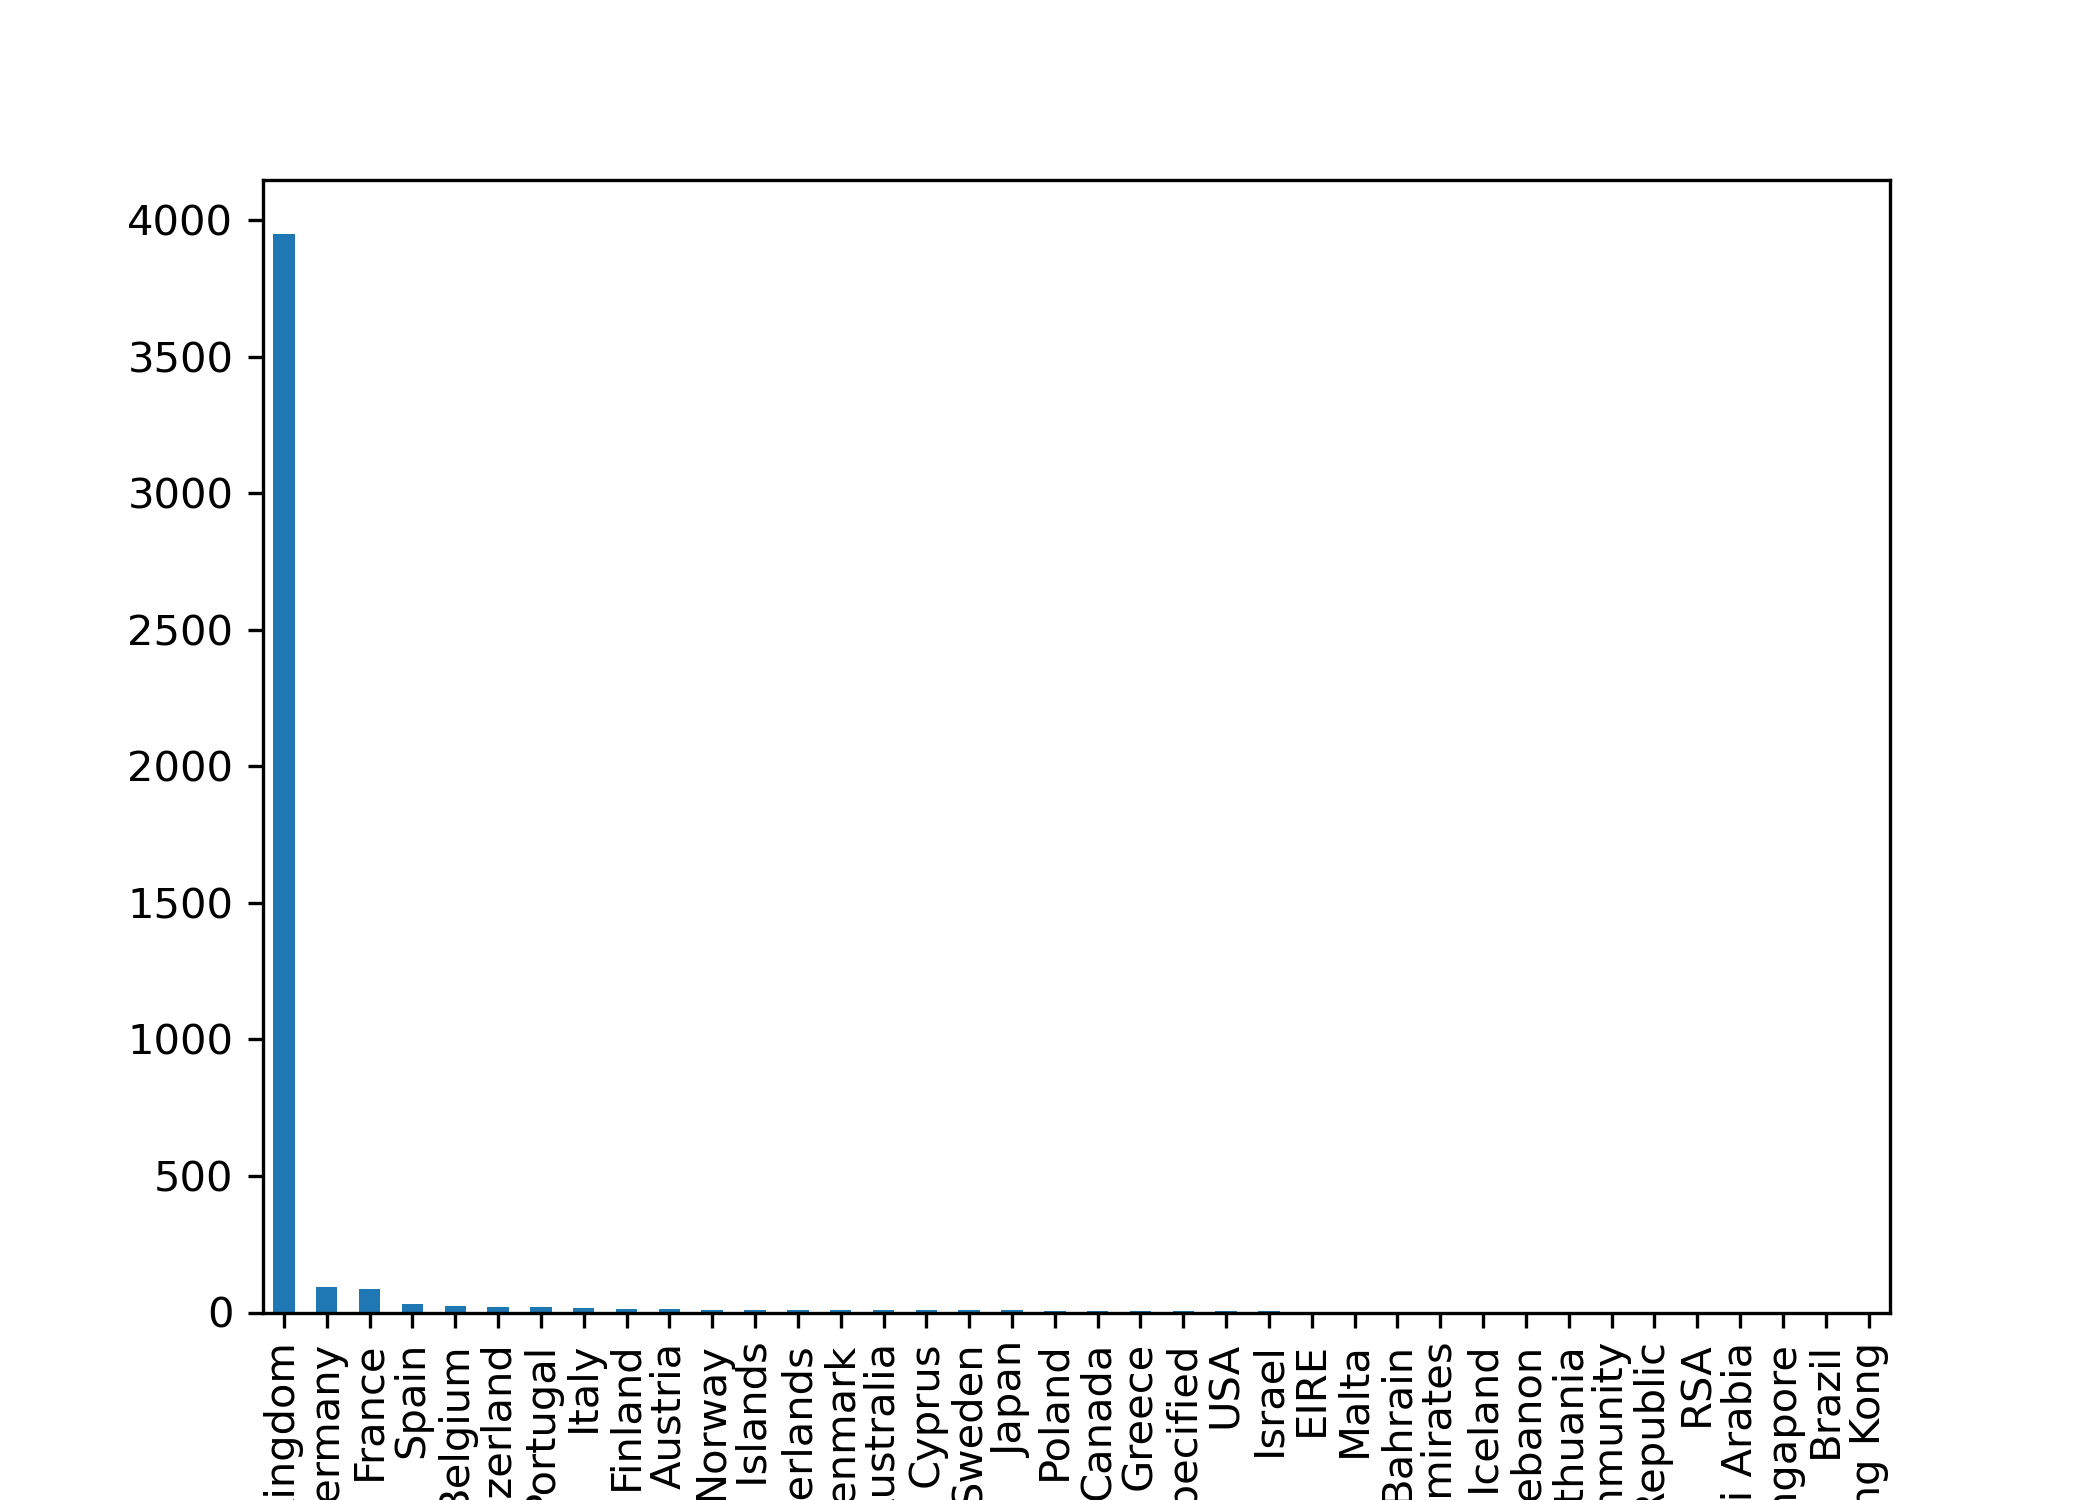
\includegraphics[width=.93\textwidth]{img/country_bar.png}
\caption{}
\label{fig:country_bar}
\end{subfigure}
\begin{subfigure}{.5\textwidth}
\centering
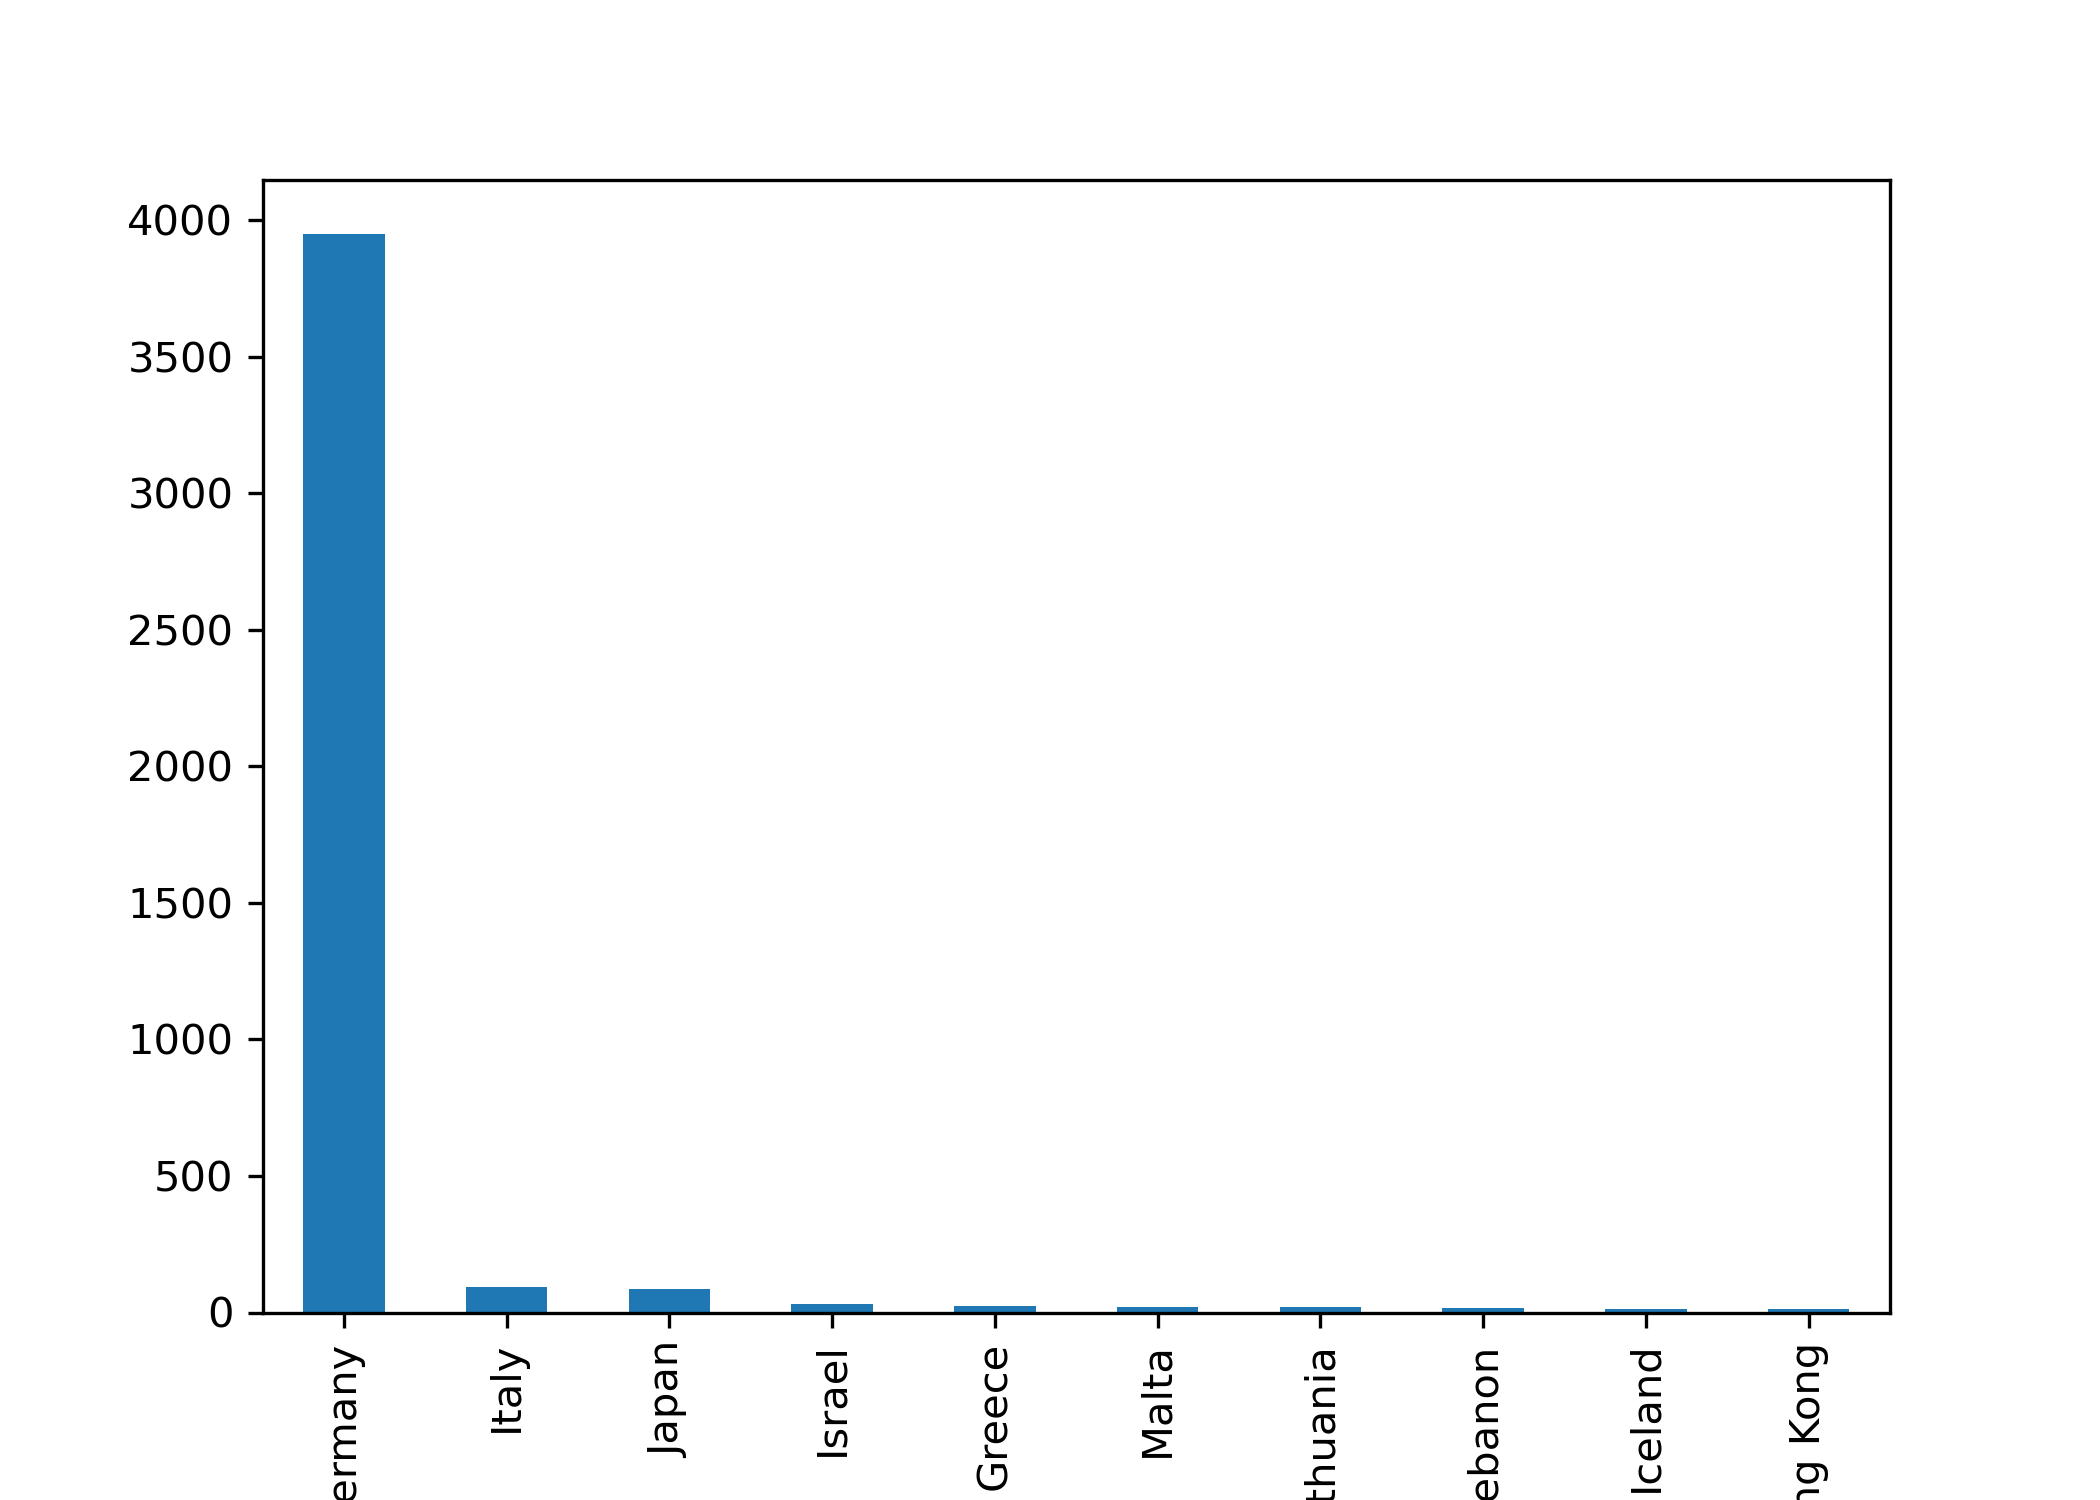
\includegraphics[width=.93\textwidth]{img/part_country_bar.png}
\caption{}
\label{fig:part_country_bar}
\end{subfigure}
\caption{CustomerCountry Distributions}
\end{figure}

Some others statistics can be visualized for the attribute \textbf{CustomerCountry}.\\
In Figure \ref{fig:country_bar}, we can see the distribution of the CustomerID with respect to the country; from the plot, it is clear that the most frequent country is the United Kingdom, that is present in about the 90\% of the rows.\\
To see also some properties of the other countries, in Figure \ref{fig:part_country_bar}, we plotted the most frequent countries, excluding the UK. Here, we can see that the second most frequent country is Germany, while the other ones are almost irrelevant, since they are in very few objects.

\begin{wrapfigure}{r}{.5\textwidth}
\centering
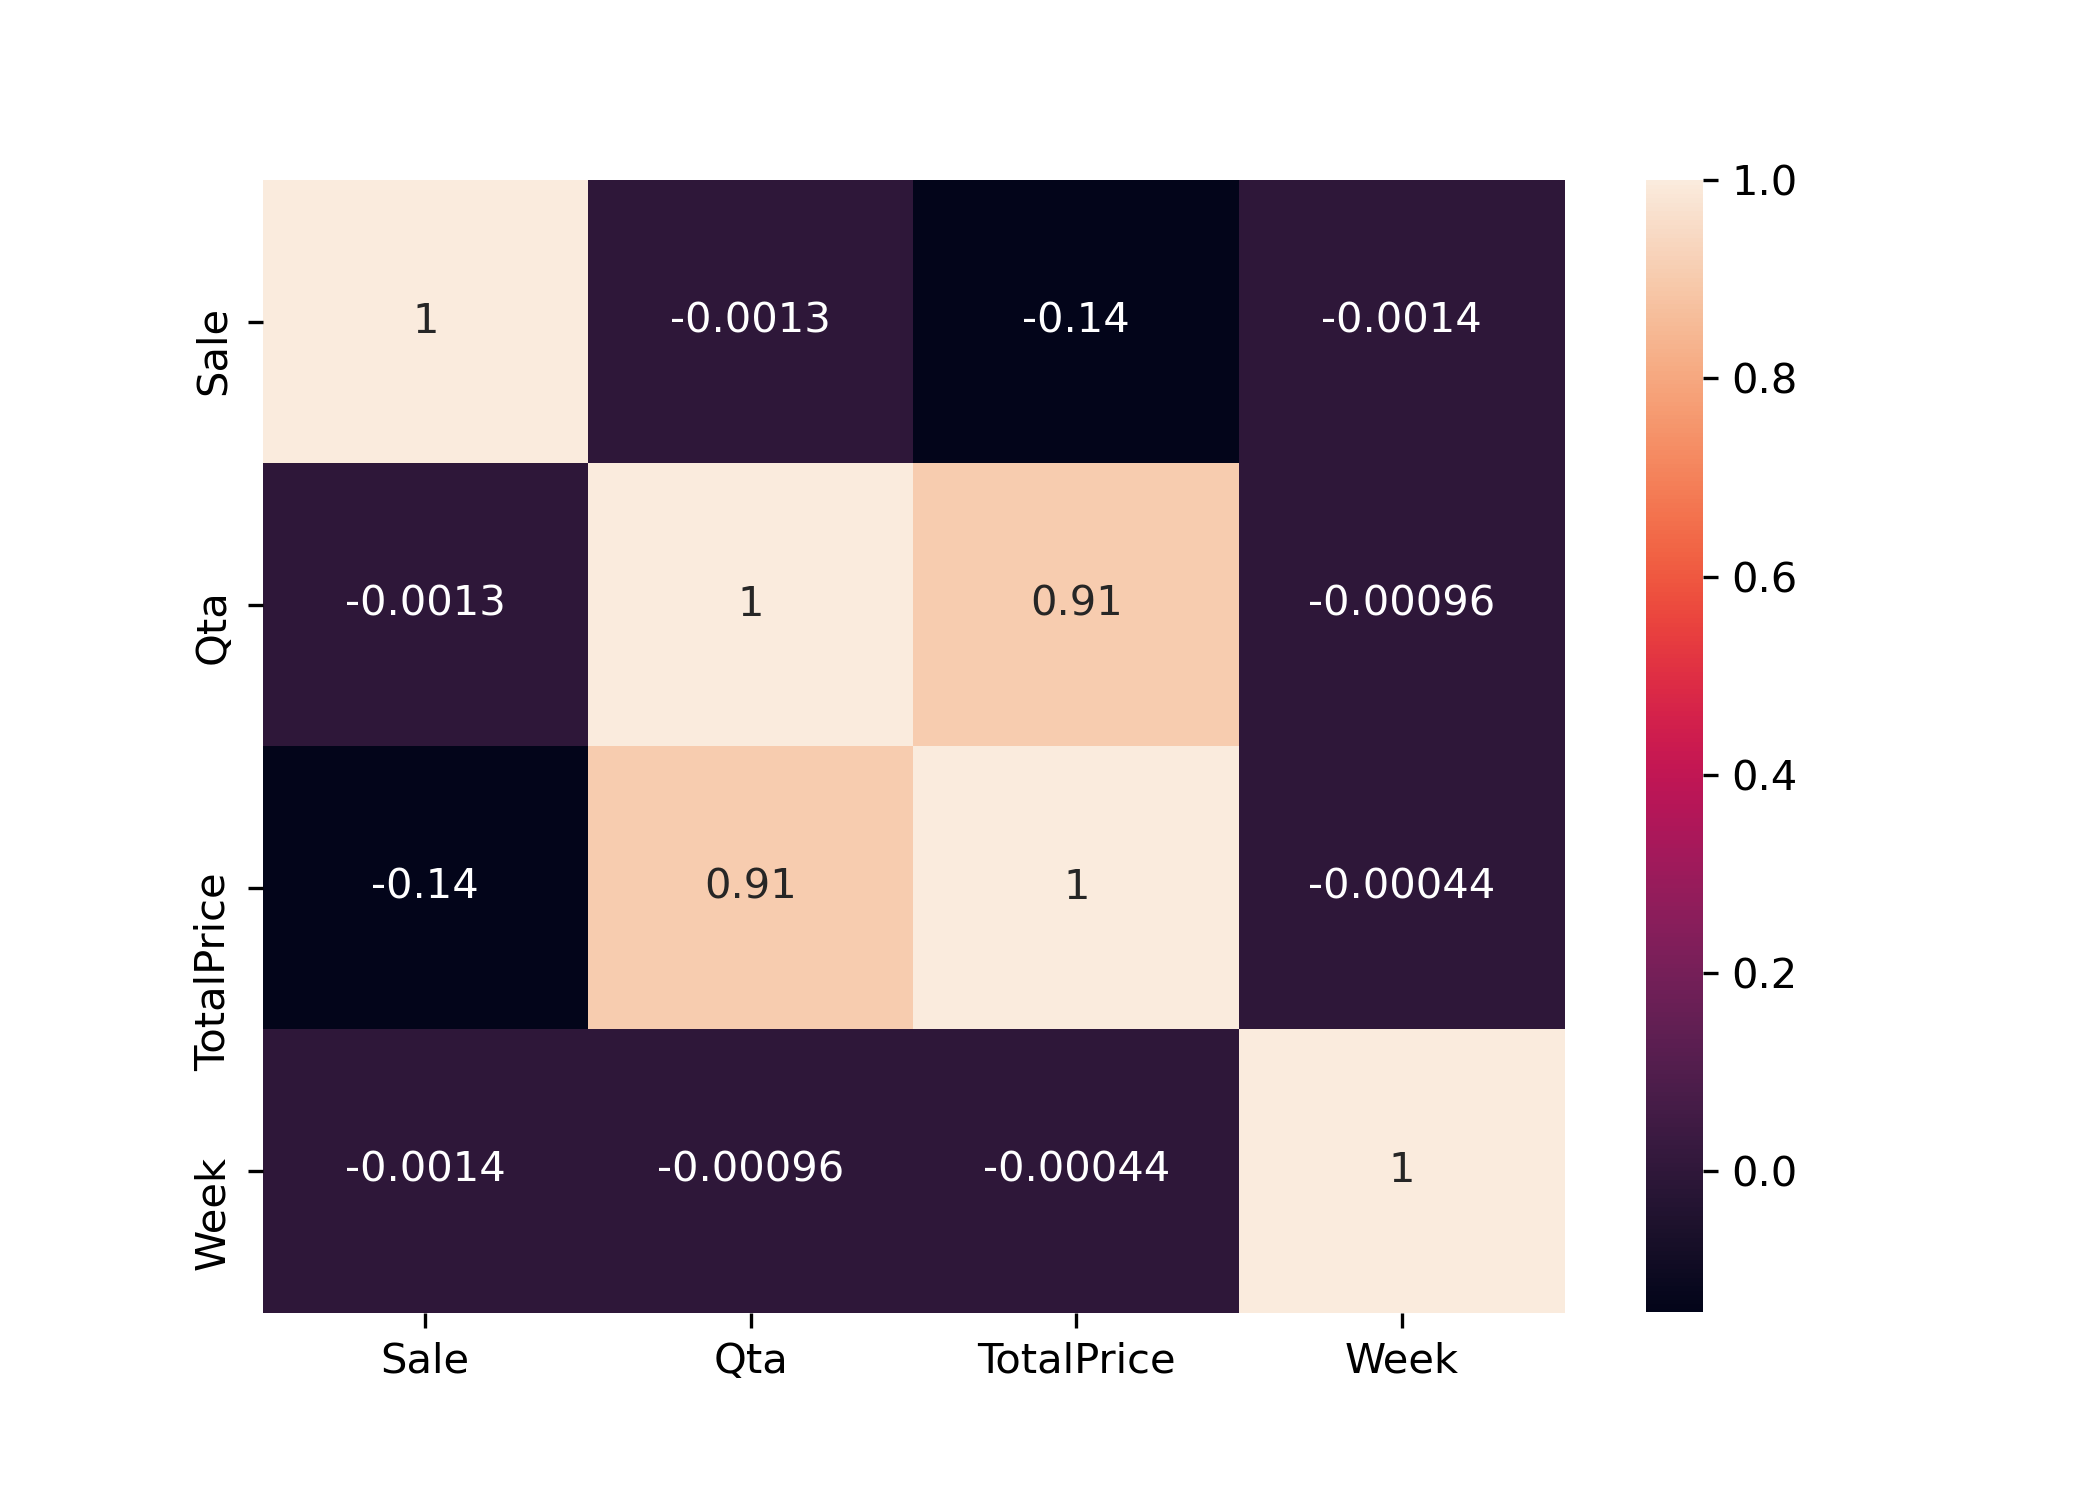
\includegraphics[width=0.49\textwidth]{img/corr.png}
\caption{Correlation Matrix}
\label{fig:corr}
\end{wrapfigure}

Finally, we see some informations about the correlation of the attributes, to see if some of them are redundant.\\
From the Figure \ref{fig:corr}, we can see that almost all the attributes are uncorrelated, except for \textbf{TotalPrice}, that shows ah high correlation with \textbf{Qta}; that follows what we expected, since \textbf{TotalPrice} is, by construction, dependent on \textbf{Qta}. So, we conclude that all the original columns are independent, and so we don't need to perform any further manipulation.
